% Options for packages loaded elsewhere
\PassOptionsToPackage{unicode}{hyperref}
\PassOptionsToPackage{hyphens}{url}
%
\documentclass[
  10pt,
  a4paper,
]{article}
\usepackage{amsmath,amssymb}
\usepackage{iftex}
\ifPDFTeX
  \usepackage[T1]{fontenc}
  \usepackage[utf8]{inputenc}
  \usepackage{textcomp} % provide euro and other symbols
\else % if luatex or xetex
  \usepackage{unicode-math} % this also loads fontspec
  \defaultfontfeatures{Scale=MatchLowercase}
  \defaultfontfeatures[\rmfamily]{Ligatures=TeX,Scale=1}
\fi
\usepackage{lmodern}
\ifPDFTeX\else
  % xetex/luatex font selection
  \setmainfont[]{DejaVu Sans}
  \setmonofont[]{DejaVu Sans Mono}
\fi
% Use upquote if available, for straight quotes in verbatim environments
\IfFileExists{upquote.sty}{\usepackage{upquote}}{}
\IfFileExists{microtype.sty}{% use microtype if available
  \usepackage[]{microtype}
  \UseMicrotypeSet[protrusion]{basicmath} % disable protrusion for tt fonts
}{}
\makeatletter
\@ifundefined{KOMAClassName}{% if non-KOMA class
  \IfFileExists{parskip.sty}{%
    \usepackage{parskip}
  }{% else
    \setlength{\parindent}{0pt}
    \setlength{\parskip}{6pt plus 2pt minus 1pt}}
}{% if KOMA class
  \KOMAoptions{parskip=half}}
\makeatother
\usepackage{xcolor}
\usepackage[margin=19mm]{geometry}
\usepackage{longtable,booktabs,array}
\usepackage{calc} % for calculating minipage widths
% Correct order of tables after \paragraph or \subparagraph
\usepackage{etoolbox}
\makeatletter
\patchcmd\longtable{\par}{\if@noskipsec\mbox{}\fi\par}{}{}
\makeatother
% Allow footnotes in longtable head/foot
\IfFileExists{footnotehyper.sty}{\usepackage{footnotehyper}}{\usepackage{footnote}}
\makesavenoteenv{longtable}
\usepackage{graphicx}
\makeatletter
\def\maxwidth{\ifdim\Gin@nat@width>\linewidth\linewidth\else\Gin@nat@width\fi}
\def\maxheight{\ifdim\Gin@nat@height>\textheight\textheight\else\Gin@nat@height\fi}
\makeatother
% Scale images if necessary, so that they will not overflow the page
% margins by default, and it is still possible to overwrite the defaults
% using explicit options in \includegraphics[width, height, ...]{}
\setkeys{Gin}{width=\maxwidth,height=\maxheight,keepaspectratio}
% Set default figure placement to htbp
\makeatletter
\def\fps@figure{htbp}
\makeatother
\setlength{\emergencystretch}{3em} % prevent overfull lines
\providecommand{\tightlist}{%
  \setlength{\itemsep}{0pt}\setlength{\parskip}{0pt}}
\setcounter{secnumdepth}{-\maxdimen} % remove section numbering
\ifLuaTeX
\usepackage[bidi=basic]{babel}
\else
\usepackage[bidi=default]{babel}
\fi
\babelprovide[main,import]{french}
\ifPDFTeX
\else
\babelfont{rm}[]{DejaVu Sans}
\fi
% get rid of language-specific shorthands (see #6817):
\let\LanguageShortHands\languageshorthands
\def\languageshorthands#1{}
\usepackage{etoolbox}
\usepackage{microtype}
\usepackage{float}
\floatplacement{figure}{H}
\sloppy
\setlength{\emergencystretch}{5em}
\AtBeginEnvironment{longtable}{\small}
\ifLuaTeX
  \usepackage{selnolig}  % disable illegal ligatures
\fi
\IfFileExists{bookmark.sty}{\usepackage{bookmark}}{\usepackage{hyperref}}
\IfFileExists{xurl.sty}{\usepackage{xurl}}{} % add URL line breaks if available
\urlstyle{same}
\hypersetup{
  pdftitle={Un opérateur commun : tête, sources et queue certifiées},
  pdfauthor={Vincent P. P. NOËL - dossier de recherche, rédaction assistée},
  pdflang={fr-FR},
  hidelinks,
  pdfcreator={LaTeX via pandoc}}

\title{Un opérateur commun : tête, sources et queue certifiées}
\usepackage{etoolbox}
\makeatletter
\providecommand{\subtitle}[1]{% add subtitle to \maketitle
  \apptocmd{\@title}{\par {\large #1 \par}}{}{}
}
\makeatother
\subtitle{Programme Riemann - V6.48 - Document 73}
\author{Vincent P. P. NOËL - dossier de recherche, rédaction assistée}
\date{13 octobre 2026}

\begin{document}
\maketitle

{
\setcounter{tocdepth}{2}
\tableofcontents
}
\hypertarget{ruxe9sultat-et-portuxe9e}{%
\section{1. Résultat et portée}\label{ruxe9sultat-et-portuxe9e}}

\textbf{Théorème local.} Pour tous les tests complexes admissibles de
\(X_S\), pour tout \(0<S\le1/2\), \[
\boxed{Q_W(f)\ge\frac1{250}\|f\|_2^2,
\qquad Q_W(f)\ge\frac1{2000}R(f).}
\] La métrique quadratique est \(R=m+\mathcal E\), avec
\(m(f)=\|f\|_2^2\). Sa racine carrée est une norme. Le domaine comprend
les fonctions de support \([-S,S]\), d'énergie finie, dont les deux
moments exponentiels s'annulent. Le certificat porte sur cet espace
infini entier. Il ne repose pas sur une liste de tests, ni sur des
données de zéros, ni sur RH.

La marge massique complète est supérieure à 0,0047. La même construction
certifie une tête polynomiale de 80 dimensions, ses sources croisées et
sa queue, pour un \textbf{minorant borné} de la forme. Les véritables
sources fortes de la forme originale ne sont pas calculées par simple
changement de nom. Les bornes plus fortes de V647 sur \(S\le3/8\)
restent disponibles.

La couverture reste bornée. Les nouveaux premiers, la règle de transport
jusqu'à l'infini, les anciennes branches, collisions et coefficient
complexe A gardent leurs questions ouvertes. Cette version établit un
raccord local exécuté ; elle ne revendique ni preuve de RH ni priorité
bibliographique.

\begin{figure}
\centering
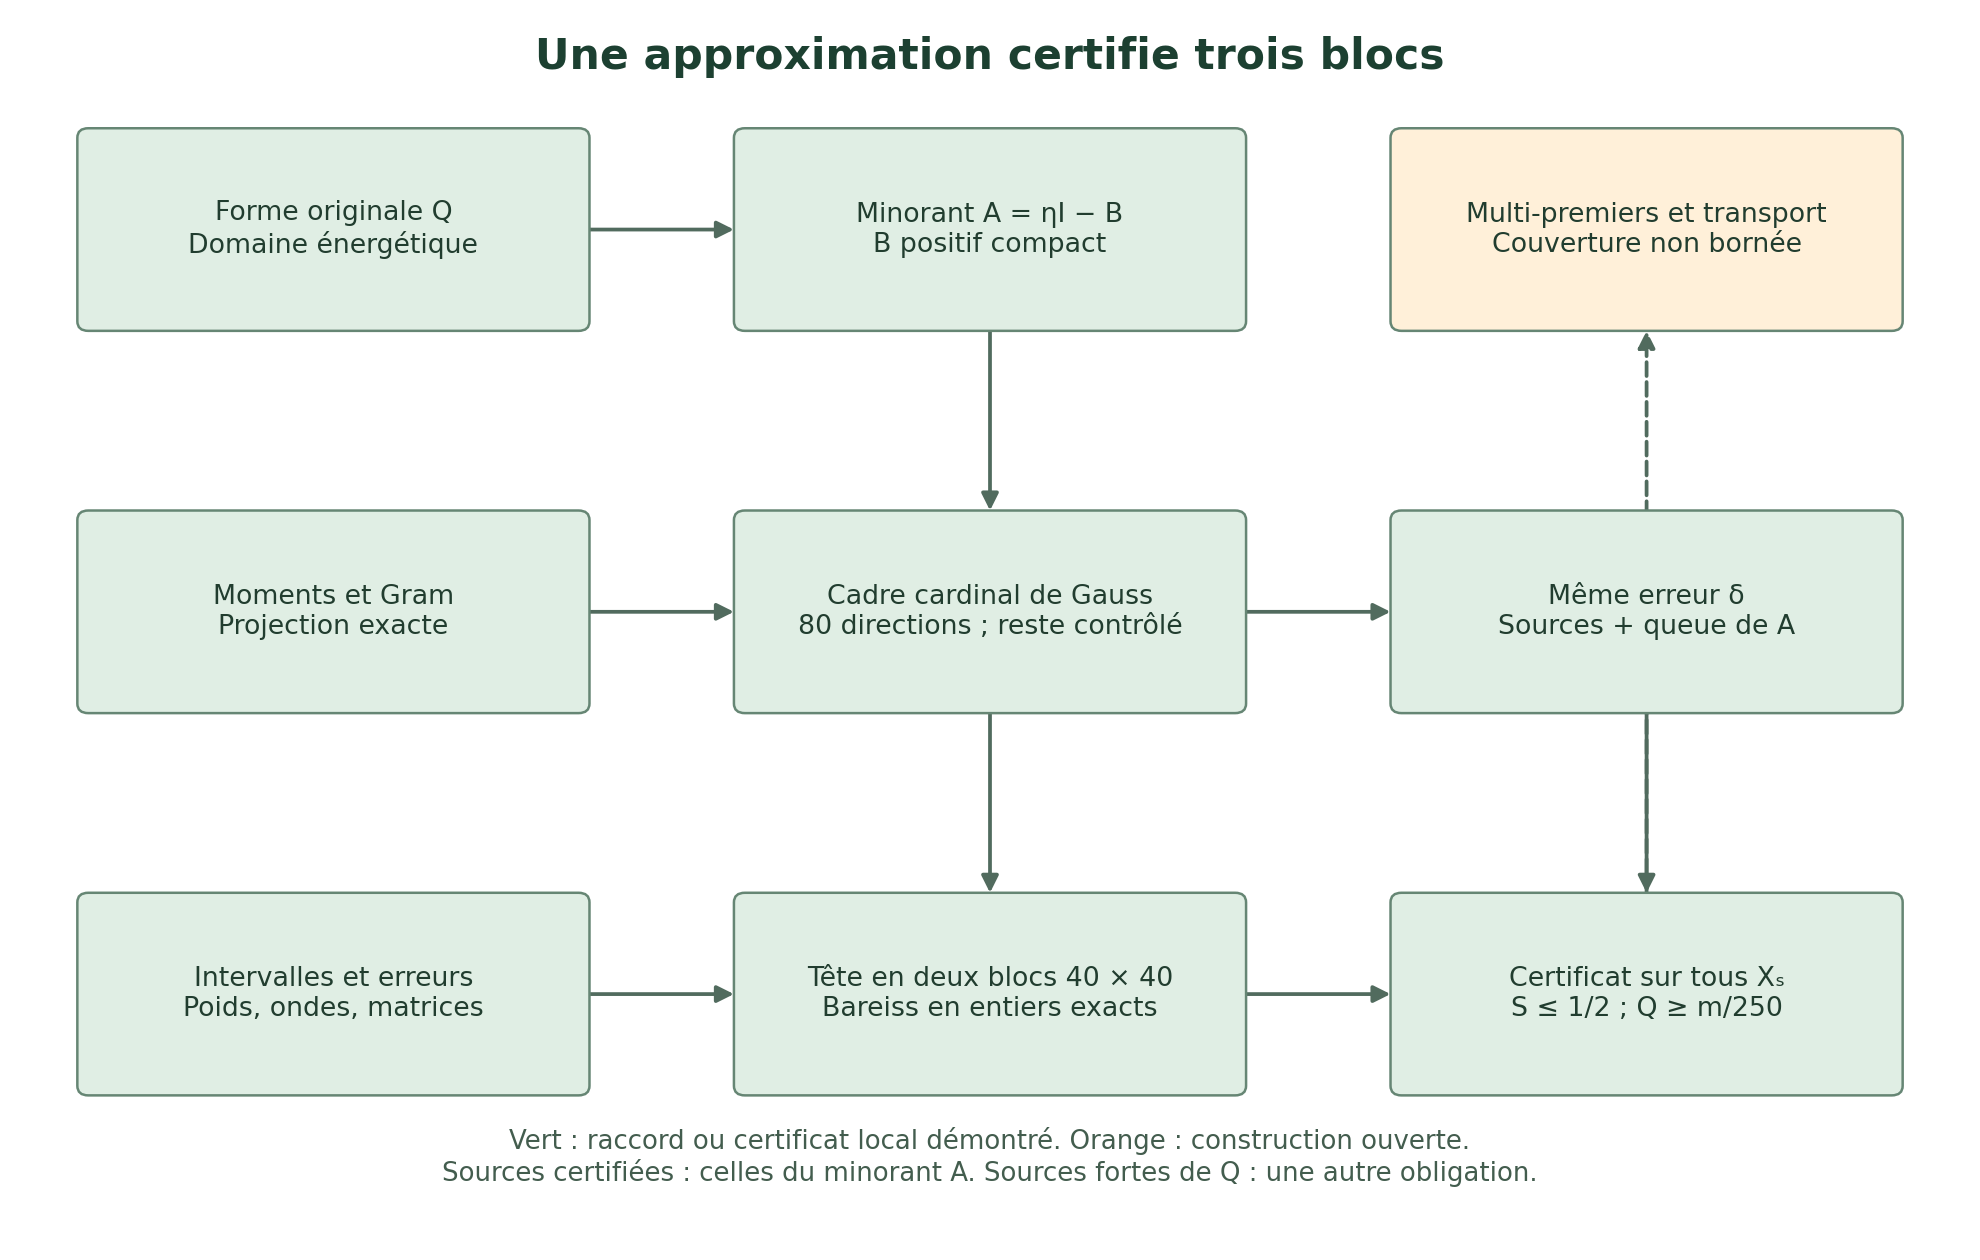
\includegraphics{73_GRAPHE_OPERATEUR_COMMUN.png}
\caption{Le même cadre fournit la tête, les sources et la queue.}
\end{figure}

\hypertarget{pourquoi-cette-repruxe9sentation-a-un-sens}{%
\section{2. Pourquoi cette représentation a un
sens}\label{pourquoi-cette-repruxe9sentation-a-un-sens}}

Le coût d'une oscillation et son accord avec un déplacement premier sont
gardés ensemble. Le plafond du coût fournit alors un opérateur compact.
On peut approcher cet opérateur par une matrice, à condition de mesurer
tout ce qui échappe à la matrice. La même erreur contrôle les directions
de queue et les attaches entre tête et queue : c'est le coup double
recherché.

Le cadre de Gauss traduit une fonction polynomiale en valeurs à des
repères avec des poids précis. Il conserve exactement les produits
scalaires des polynômes concernés. Les valeurs aux repères seules ne
donnent aucune garantie sur une fonction quelconque : le reste
d'interpolation fournit le pont vers tout l'espace.

\begin{longtable}[]{@{}
  >{\raggedright\arraybackslash}p{(\columnwidth - 4\tabcolsep) * \real{0.3333}}
  >{\raggedright\arraybackslash}p{(\columnwidth - 4\tabcolsep) * \real{0.3333}}
  >{\raggedright\arraybackslash}p{(\columnwidth - 4\tabcolsep) * \real{0.3333}}@{}}
\toprule\noalign{}
\begin{minipage}[b]{\linewidth}\raggedright
Traduction
\end{minipage} & \begin{minipage}[b]{\linewidth}\raggedright
Conservé
\end{minipage} & \begin{minipage}[b]{\linewidth}\raggedright
Erreur ou garde
\end{minipage} \\
\midrule\noalign{}
\endhead
\bottomrule\noalign{}
\endlastfoot
Fourier unitaire & Masse, phases et forme exacte & Intégration en
\(dt\), sans facteur supplémentaire \\
Projection des moments & Toutes les directions admissibles & Gram de la
métrique L² \\
Minorant borné & Implication suffisante vers le signe & Les sources
exactes de Q ne sont pas identiques \\
Cadre cardinal de Gauss & Gram des polynômes, exactement & Nœuds, poids
et reste à certifier \\
Matrice vers opérateur & Majorant de la plus grande valeur & Erreur en
norme opérateur sur tout l'espace \\
Inclusion des supports & Moments et formes globales & Seulement les
supports sous le plafond certifié \\
\end{longtable}

Les coefficients opératoires sont sans dimension. Les amplitudes portent
\(A_{\rm amp}\), et \(m,\mathcal E,Q_W,R\) portent \(A_{\rm amp}^2\). Ce
suivi d'unités est une arithmétique de types, sans énergie physique ni
variable temporelle supposée.

\hypertarget{l1-l2-identituxe9-conjointe-et-projection}{%
\section{3. L1-L2 : identité conjointe et
projection}\label{l1-l2-identituxe9-conjointe-et-projection}}

\textbf{Lemme L1.} À \(S=1/2\), seul le premier 2 agit. Avec la Fourier
unitaire, \[
\widehat f(t)=(2\pi)^{-1/2}\int f(x)e^{-itx}dx,
\quad w_2=\frac{\log2}{\sqrt2},\quad
C_0=\log(8\pi)+\gamma_E+\frac\pi2,
\] \[
a(t)=\sum_{n\ge0}\frac{2t^2}{b_n(b_n^2+t^2)},\quad b_n=2n+\frac12,
\qquad b(t)=a(t)+2w_2(1-\cos(t\log2)),
\] on a \[
Q_W(f)=\int_{\mathbb R}b(t)|\widehat f(t)|^2dt-(C_0+2w_2)m(f).
\] \textbf{Preuve.} Plancherel transforme les différences de
translations en \(2(1-\cos(td))\). L'expansion positive du poids
\(e^{-d/2}/(1-e^{-2d})\) donne \(a\). Le déplacement premier a le
multiplicateur \(\cos(t\log2)\). La condition \(2S=1<\log3\) exclut les
autres premiers. Ajouter puis soustraire \(2w_2m\) donne l'identité.

\textbf{Lemme L2.} Soit \(P_W=I-\Pi_W\), où
\(W=\operatorname{span}\{\cosh(x/2),\sinh(x/2)\}\). Le Gram est \[
G_W=\operatorname{diag}(S+\sinh S,\sinh S-S).
\] Les ondes projetées sont \(r_{+,t}=P_W\cos(tx)\) et
\(r_{-,t}=P_W\sin(tx)\). Les parités se séparent sans couplage. Les
tests admissibles sont conservés par \(P_W\). \textbf{Preuve.} Les deux
générateurs sont orthogonaux par parité. L'intégration de leurs carrés
donne le Gram. Les moments nuls signifient exactement \(f\perp W\). Tous
les produits de parités opposées ont une intégrale nulle. Les mêmes
relations valent sur les espaces complexifiés.

Les moments des ondes, notés \(c(t),s(t)\), viennent de \[
z_S(t)=\frac{2\sinh((1/2+it)S)}{1/2+it},\quad
c(t)=\Re z_S(t),\quad s(t)=\Im z_S(t).
\] Le programme les évalue par des formules réelles et le Gram exact. Il
ne substitue pas le Gram d'une grille à ce Gram des moments.

\hypertarget{l3-un-minorant-bornuxe9-identituxe9-moins-compact}{%
\section{4. L3 : un minorant borné, identité moins
compact}\label{l3-un-minorant-bornuxe9-identituxe9-moins-compact}}

\textbf{Lemme L3.} Posons \(U=8\), \(\phi_U=(U-b)_+\). Dans chaque
parité, \[
B_U=\frac1\pi\int_0^\infty\phi_U(t)
|r_t\rangle\langle r_t|dt,
\qquad A_U=(U-C_0-2w_2)I-B_U.
\] Alors \(Q_W(f)\ge\langle f,A_Uf\rangle\) sur son domaine. L'opérateur
\(B_U\) est positif, compact, à noyau lisse. \textbf{Preuve.}
\(b\ge\min(b,U)=U-(U-b)_+\), puis la Fourier et la parité fournissent le
facteur \(1/\pi\). Le multiplicateur \(a\) est croissant et tend vers
l'infini ; le poids \(\phi_U\) a donc un support fréquentiel compact.
L'intégrale d'opérateurs positifs de rang un a une trace finie. Son
noyau est lisse car les fréquences sont bornées.

La série positive et sa queue par intégrale donnent effectivement \[
a(90)\in[8{,}0340523942,\,8{,}0341691405].
\] Puisque \(b\ge a\), toutes les contributions au-delà de \(T=90\) sont
nulles. Il s'agit d'une exclusion globale certifiée, pas du minimum
observé sur une grille finie.

L'intégration des opérateurs conserve le même test dans toutes les
couches. La norme d'une somme peut être plus petite que la somme des
normes, dont les directions maximales pourraient différer. V647
démontrait ce pont ; cette version certifie sa norme sur un espace
complet.

\hypertarget{l4-le-cadre-cardinal-de-gauss}{%
\section{5. L4 : le cadre cardinal de
Gauss}\label{l4-le-cadre-cardinal-de-gauss}}

\textbf{Lemme L4.} Soient \(\xi_i\) les racines du polynôme de Legendre
\(p_N\), \(x_i=S\xi_i\), et \(w_i\) les poids de Gauss sur \([-S,S]\).
Si \(l_i(x_j)=\delta_{ij}\) sont les polynômes cardinaux, alors \[
\int l_i(x)l_j(x)dx=w_i\delta_{ij}.
\] Les fonctions \(l_i/\sqrt{w_i}\) constituent une base orthonormale de
l'espace polynomial de degré inférieur à \(N\). Le vecteur de
coordonnées de l'interpolant d'une fonction \(r\) est
\((\sqrt{w_i}r(x_i))_i\). \textbf{Preuve.} Gauss intègre exactement tout
polynôme de degré au plus \(2N-1\). Le produit de deux cardinaux a degré
au plus \(2N-2\). L'évaluer aux nœuds donne immédiatement le Gram
diagonal. La symétrie des nœuds sépare les deux parités ; avec \(N=80\),
chaque bloc a dimension 40.

Les nœuds proposés numériquement sont certifiés par des changements de
signe \textbf{exacts en entiers}. Quarante intervalles positifs
disjoints, reflétés par parité, donnent 80 racines distinctes d'un
polynôme de degré 80 ; chaque intervalle contient donc exactement une
racine. Les poids sont encadrés par \[
w_i=\frac{2S}{(1-\xi_i^2)p_N'(\xi_i)^2}.
\] La dérivée est évaluée rationnellement au centre de l'intervalle. La
borne \(|p_N''|\le N^4\), issue de l'inégalité de Markov et de
\(|p_N|\le1\), encadre sa variation. Cela évite l'élargissement excessif
d'une récurrence intervalle près d'une racine. Les valeurs décimales de
Nyström ne constituent aucune prémisse de précision.

Si \(I_N\) désigne l'interpolation et \(L_N=(2N)!/[2^N(N!)^2]\) le
coefficient dominant de \(p_N\), \[
\left|\prod_i(x-x_i)\right|\le\frac{S^N}{L_N}.
\] Le reste de Lagrange des ondes réelles est donc majoré par
\((TS)^N/(N!L_N)\). Les dérivées oscillantes ont module au plus \(T^N\)
; aucun facteur \(e^{TS}\) n'est ajouté. Les générateurs exponentiels
donnent une correction avec \(e^{S/2}(S/2)^N\). À \(S=1/2\),
\(\sinh(1/2)-1/2>1/48\) et \(e^{1/4}<4/3\), d'où \[
\|r_t-I_Nr_t\|_2\le\varepsilon_N
=\frac{45^N+(28/3)(1/4)^N}{N!L_N},\quad N=80.
\] \textbf{Preuve.} Appliquer le reste aux ondes puis aux deux
générateurs. Le coefficient de leur projection est majoré par Cauchy, au
plus \(\sqrt{48}<7\). Le produit avec \(e^{1/4}\) est inférieur à
\(28/3\).

On interpole les ondes \textbf{après} leur projection sur les moments.
Les deux projections ne sont pas supposées commuter. La tête polynomiale
appartient au L² ambiant ; ses vecteurs n'ont pas à appartenir au
domaine énergétique de Q, puisqu'on n'y évalue que l'opérateur borné B.

\hypertarget{l5-aucune-erreur-ne-disparauxeet-dans-la-traduction}{%
\section{6. L5 : aucune erreur ne disparaît dans la
traduction}\label{l5-aucune-erreur-ne-disparauxeet-dans-la-traduction}}

\textbf{Lemme L5.} Si l'approximation des ondes a une erreur uniforme
\(\varepsilon\) en L² et si \(\|r_t\|\le1\), le changement de
l'opérateur pondéré est au plus \[
\frac{UT}{\pi}(2\varepsilon+\varepsilon^2).
\] \textbf{Preuve.} La différence de deux produits de rang un a une
norme au plus \((\|r\|+\|v\|)\|r-v\|\). Intégrer et utiliser
\(0\le\phi\le U\). La même formule, avec \(1+\varepsilon_N\), couvre
l'évaluation de l'interpolant déjà approché.

Le poids est construit à partir d'une table encadrée de b, au pas
\(H=1/100\). Ses valeurs centrales sont quantifiées à \(2^{-44}\), puis
interpolées \textbf{en entiers exacts}. Les dérivées vérifient \[
|b'|<13/2,\qquad |b''|<33.
\] Pour les établir, on dérive la série positive :
\(\sup a'\le(21/16)\sum b_n^{-2}\), \(\sum b_n^{-2}\le109/25\), et
\(\sup|a''|\le4\sum b_n^{-3}\le32{,}416\). La phase première ajoute
moins de 0,7 et 0,49 respectivement.

Si \(r_{\rm tab}\) est l'erreur maximale des valeurs tabulées, le poids
constant aux milieux du pas fréquentiel \(h=1/1000\) s'écarte du vrai
poids d'au plus \[
\delta_\phi=r_{\rm tab}+33H^2/8+(13/2)h/2.
\] La partie positive est 1-lipschitzienne. Plancherel et la contraction
de \(P_W\) donnent une erreur \textbf{opératoire} au plus
\(\delta_\phi\), sans facteur \(T/\pi\).

Pour le poids constant de chaque cellule, l'erreur des milieux de
\(|r_t\rangle\langle r_t|\) est majorée par \[
\delta_{\rm milieux}\le
\frac{(47/15)S^3\,UT\,h^2}{24\pi}.
\] On utilise la borne sur la dérivée seconde de ce produit de rang un,
comme dans V647. Le poids constant est borné entre 0 et U ; cette garde
est testée.

Les sinus et cosinus sont évalués par Taylor sur \(z/64\), puis six
doublements d'angle. Les coefficients, les opérations et les restes sont
encadrés vers l'extérieur. Les exponentielles des générateurs sont
traitées par Taylor de degré 24. Les intervalles des nœuds et de leurs
poids entrent dans les \textbf{vecteurs pondérés}, avant calcul de leur
erreur L². Le certificat n'utilise ni les sinus de NumPy ni la digamma
flottante.

La multiplication matricielle binaire64 a son propre budget. Avec
\(u=2^{-53}\), \(n_f=90\,000\), \[
\gamma_k=\frac{ku}{1-ku},\quad k=2n_f+128,\qquad
\delta_{\rm matrice}\le32\gamma_kUT/\pi.
\] \textbf{Justification.} Sous opérations IEEE correctement arrondies,
un produit de k facteurs d'erreur s'écarte de 1 d'au plus \(\gamma_k\).
La longueur choisie domine les produits, sommes, poids et accumulations
par blocs. Les produits absolus sont dominés par les sommes de normes
des colonnes ; la garde de norme et le facteur 32 couvrent ces sommes.
La symétrisation et la quantification matricielle ont aussi leur erreur
explicite. Ce modèle arithmétique est déclaré ; le format binaire64 et
des cas de contrôle de l'arrondi au plus proche sont vérifiés ; il ne
constitue pas une vérification formelle du compilateur ou du matériel.

\begin{longtable}[]{@{}ll@{}}
\toprule\noalign{}
Erreur opératoire certifiée & Majorant décimal indicatif \\
\midrule\noalign{}
\endhead
\bottomrule\noalign{}
\endlastfoot
Poids conjoint et cellules & 0.00372087309 \\
Milieux du noyau & 3.74014116e-06 \\
Interpolation spatiale & 1.52014444e-07 \\
Arrondis matriciels & 1.4666418e-07 \\
Vecteurs pondérés, bloc pair & 1.16287242e-10 \\
Total, bloc pair & 0.00372491202 \\
\end{longtable}

\hypertarget{l6-le-plafond-matriciel-devient-un-plafond-infini}{%
\section{7. L6 : le plafond matriciel devient un plafond
infini}\label{l6-le-plafond-matriciel-devient-un-plafond-infini}}

\textbf{Lemme L6.} La matrice quantifiée \(M_N\) est rationnelle et
symétrique. Le calcul entier de Bareiss vérifie \[
\tau_+I-M_{N,+}\succ0,\quad \tau_+=1{,}63860;
\qquad \tau_-I-M_{N,-}\succ0,\quad \tau_-=1{,}48237.
\] Alors \(\lambda_{\max}(M_N)<\tau\). Si l'erreur totale en norme de
l'opérateur est au plus \(\delta\), \[
\|B_U\|\le\tau+\delta.
\] \textbf{Preuve.} Les déterminants principaux calculés par Bareiss
sont positifs, avec toutes les divisions exactes ; le critère de
Sylvester prouve les inégalités. Le solveur flottant ne propose que les
plafonds candidats. Pour tout vecteur, la forme de B est majorée par
celle de sa matrice plus \(\delta\|f\|^2\). B étant positif, cela majore
sa norme entière. Une éventuelle petite valeur négative de la matrice
arrondie ne change pas cette argumentation.

\begin{longtable}[]{@{}lll@{}}
\toprule\noalign{}
Quantité certifiée & Pair & Impair \\
\midrule\noalign{}
\endhead
\bottomrule\noalign{}
\endlastfoot
Norme B, majorant & 1.642324912 & 1.486094912 \\
Erreur totale δ & 0.003724912 & 0.003724912 \\
Marge massique sur les deux blocs & 0.004745324 & même borne \\
Marge dans R sur les deux blocs & 0.000690978 & même borne \\
\end{longtable}

\hypertarget{l7-signe-r-et-tous-les-sous-supports}{%
\section{8. L7 : signe, R et tous les
sous-supports}\label{l7-signe-r-et-tous-les-sous-supports}}

\textbf{Lemme L7.} Avec \(C_1=C_0+2w_2\), le budget certifié donne
\(c=U-C_1-\max(\tau_\pm+\delta_\pm)>0{,}0047\). Donc \(Q_W\ge cm\). Les
bandes du déplacement log2 sont disjointes à ce support ; Cauchy donne
\(|Q_{\rm pr}|\le w_2m\), puis \(Q_W\ge\mathcal E-(C_0+w_2)m\). En
notant \(L=C_0+w_2\), \[
Q_W\ge\frac{c}{c+L+1}R.
\] \textbf{Preuve.} \(m\le Q_W/c\) et \(\mathcal E\le Q_W+Lm\).
Additionner et réarranger donne la formule. Les constantes lisibles
\(c\ge1/250\), \(L<6\) entraînent \(Q_W\ge R/1751\ge R/2000\). Le
prolongement par zéro conserve les moments et les formes globales ; tous
les domaines \(X_S\), \(S\le1/2\), sont inclus dans le domaine certifié.
Les meilleures constantes déjà prouvées sur les supports plus petits
conservent leur portée.

\hypertarget{l8-tuxeate-sources-et-queue-du-muxeame-minorant}{%
\section{9. L8 : tête, sources et queue du même
minorant}\label{l8-tuxeate-sources-et-queue-du-muxeame-minorant}}

\textbf{Lemme L8.} Soit \(\Pi_N\) la projection orthogonale sur le cadre
polynomial, et \(\widetilde B_N\) l'opérateur de matrice \(M_N\) dans sa
base orthonormale. La même borne \(\|B_U-\widetilde B_N\|\le\delta\)
donne \[
\begin{aligned}
\|\Pi_NB_U\Pi_N\|&\le\tau+\delta,\\
\|(I-\Pi_N)B_U(I-\Pi_N)\|&\le\delta,\\
\|(I-\Pi_N)B_U\Pi_N\|&\le\delta.
\end{aligned}
\] Pour les sources \(\rho_i=(I-\Pi_N)B_Ue_i\), \[
\operatorname{Gram}(\rho_i)\preceq\delta^2 I.
\] \textbf{Preuve.} Les blocs de queue et croisés de \(\widetilde B_N\)
sont nuls. Chaque bloc de la différence est donc une contraction de
cette différence. Le Gram des colonnes est le carré du bloc croisé.
L'identité exige une base orthonormale ; une autre base demande son Gram
de tête.

Dans la métrique L² du minorant, posons \(\eta=U-C_1\). La tête de
\(A_U\) a un plancher \(\eta-\tau-\delta\), la queue a un plancher
\(\eta-\delta>0\), et le Schur satisfait \[
\mathcal G_N\succeq
\left(\eta-\tau-\delta-\frac{\delta^2}{\eta-\delta}\right)I.
\] Les trois bornes sont réellement assemblées en fractions exactes.

\begin{longtable}[]{@{}lll@{}}
\toprule\noalign{}
Contrat du minorant A & Pair & Impair \\
\midrule\noalign{}
\endhead
\bottomrule\noalign{}
\endlastfoot
Plancher de queue L² & 1.643345324 & 1.643345324 \\
Dette opératoire de Schur & 0.000008443 & 0.000008443 \\
Marge de Schur & 0.004736880 & 0.160966880 \\
\end{longtable}

La tête finie, les sources et la queue sont donc certifiées ensemble
pour \(A_U\). Cela fournit une seconde vérification du raccord de signe.
La différence \(Q_W-A_U\) est positive, généralement non bornée : le
signe suffisant se transporte vers Q, mais les sources exactes de Q ne
sont pas celles de A. La norme opératoire L² suffit pour B ; le
transport général de Q conserve ses exigences propres de norme de
graphe.

\hypertarget{les-quatre-portes-et-la-suite}{%
\section{10. Les quatre portes et la
suite}\label{les-quatre-portes-et-la-suite}}

\begin{longtable}[]{@{}
  >{\raggedright\arraybackslash}p{(\columnwidth - 4\tabcolsep) * \real{0.3333}}
  >{\raggedright\arraybackslash}p{(\columnwidth - 4\tabcolsep) * \real{0.3333}}
  >{\raggedright\arraybackslash}p{(\columnwidth - 4\tabcolsep) * \real{0.3333}}@{}}
\toprule\noalign{}
\begin{minipage}[b]{\linewidth}\raggedright
Porte
\end{minipage} & \begin{minipage}[b]{\linewidth}\raggedright
Ce qui est acquis
\end{minipage} & \begin{minipage}[b]{\linewidth}\raggedright
Ce qui reste à construire
\end{minipage} \\
\midrule\noalign{}
\endhead
\bottomrule\noalign{}
\endlastfoot
Arithmétique & Compensation du premier2 conservée et certifiée
jusqu'à1/2 & Coût conjoint multi-premiers et loi de signe couvrante \\
Tête praticable & Cadre exact de Gauss ; 40 dimensions par parité &
Cadres et plafonds opératoires lorsque de nouveaux premiers entrent \\
Couplages & Sources du minorant, Gram et dette de Schur certifiés &
Sources fortes de Q dans la méthode générale ; transport entre
supports \\
Couverture & Tous \(0<S\le1/2\) & Une famille non bornée, nouveaux
premiers et convergence \\
\end{longtable}

La prochaine construction porte sur le \textbf{coût conjoint
multi-premiers}, avec les mêmes tests de traduction et la même brique
d'erreur opératoire. L'objectif est un principe de compensation et de
transport ; allonger seulement la liste des supports ne fournit pas ce
principe. Le pilote de Bellman historique reste documentaire : aucun
score ne mesure ici une probabilité de démontrer RH.

\hypertarget{vuxe9rification-et-ruxe9fuxe9rences}{%
\section{11. Vérification et
références}\label{vuxe9rification-et-ruxe9fuxe9rences}}

Les paramètres ont été choisis après exploration, puis figés avant
validation : \(S=1/2\), \(U=8\), \(T=90\), \(N=80\), \(h=1/1000\),
\(H=1/100\), 256 termes de série, 160 bits pour les intervalles
scalaires et 44 bits fixes pour les tables et matrices. Le journal
conserve le protocole, son empreinte, le code, les nœuds, poids, tables,
matrices entières et déterminants principaux.

Références primaires : \href{https://dlmf.nist.gov/3.5\#v}{NIST DLMF
3.5(v)}, quadrature de Gauss ; \href{https://dlmf.nist.gov/18.3}{DLMF
18.3}, polynômes orthogonaux ;
\href{https://numpy.org/doc/stable/reference/generated/numpy.finfo.html}{NumPy
finfo}, format binaire64. Les identités de Weil et les ponts précédents
sont démontrés dans les documents 71 et 72. Ce texte est préparé pour
relecture, sans publication extérieure ni vérification formelle
automatisée annoncée.

Reproduction depuis \texttt{3\_Preuves\_et\_calculs} : lancer
\texttt{python\ scripts/v648\_common\_certificate\_experiment.py}, puis
\texttt{python\ tests/run\_all\_tests.py}. Le diagnostic séparé est
\texttt{scripts/v648\_common\_operator\_diagnostic.py}. Les résultats
sont dans \texttt{data/v648\_common\_certificate\_resultats.json} ; le
protocole dans \texttt{data/v648\_protocole\_operateur\_commun.json}.

\end{document}
